\subsection[Przegląd protokołów wykorzystywanych w IoT]{Przegląd protokołów wykorzystywanych w IoT}
\begin{itemize}
    \item Message Queue Telemetry Transport (MQTT) - Protokół MQTT jest lekkim protokołem transmisji danych, umożliwia komunikację między systemami za pośrednictwem serwera. MQTT jest oparty o wzorzec Publish-Subscribe, wzorzec ten mówi, że wiadomość od nadawcy nie trafia bezpośrednio do odbiorcy tylko najpierw trafia do serwera pośredniczącego (eng. broker). Dzięki serwerowi pośredniczącemu odbiorca nic nie wie o osobie która nadaj wiadomość oraz nie dostaje potwierdzenia o doręczonej wiadomości. Plusami protokołu MQTT jest na pewno prędkość przesyłania danych, zawdzięcza to dzięki małemu narzutowi na transportowane dane, dodatkowo zapewnia bardzo wysoką niezawodność transmisji, dlatego idealnie sprawdza się przy połączeniach między dwoma urządzeniami. Kolejną zaletą protokołu MQTT jest możliwość komunikacji dwukierunkowej oznacza to, że klient MQTT może być równocześnie subskrybentem jak i publisherem.
\end{itemize}
\begin{figure}[H]
    \centering
    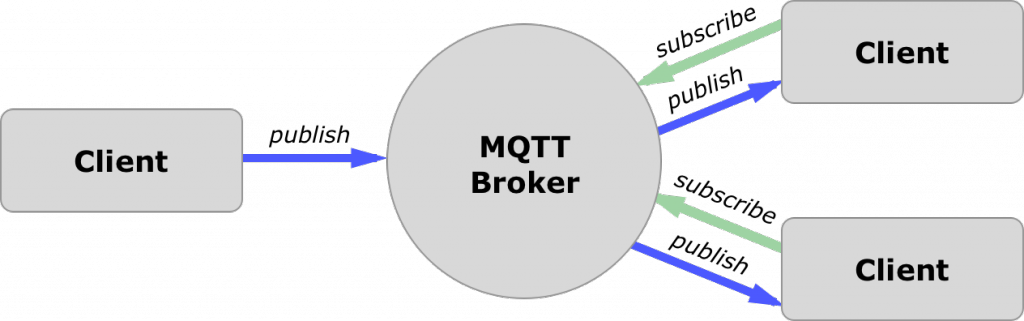
\includegraphics[width=\textwidth]{kp04}
    \caption{Placeholder}
    \label{fig:iotarch}
\end{figure}
\begin{itemize}
    \item WebSocket jest protokołem opartym na TCP, tak jak MQTT zapewnia komunikację dwukierunkową. Po zestawieniu połączenia zarówno serwer jak i urządzenie mogą w dowolnym momencie wymieniać się danymi. WebSocket jest dużo lepszym rozwiązaniem od np. long polling, ponieważ mogą obsłużyć w tym samym czasie większą ilość zapytań.
\end{itemize}
\begin{figure}[H]
    \centering
    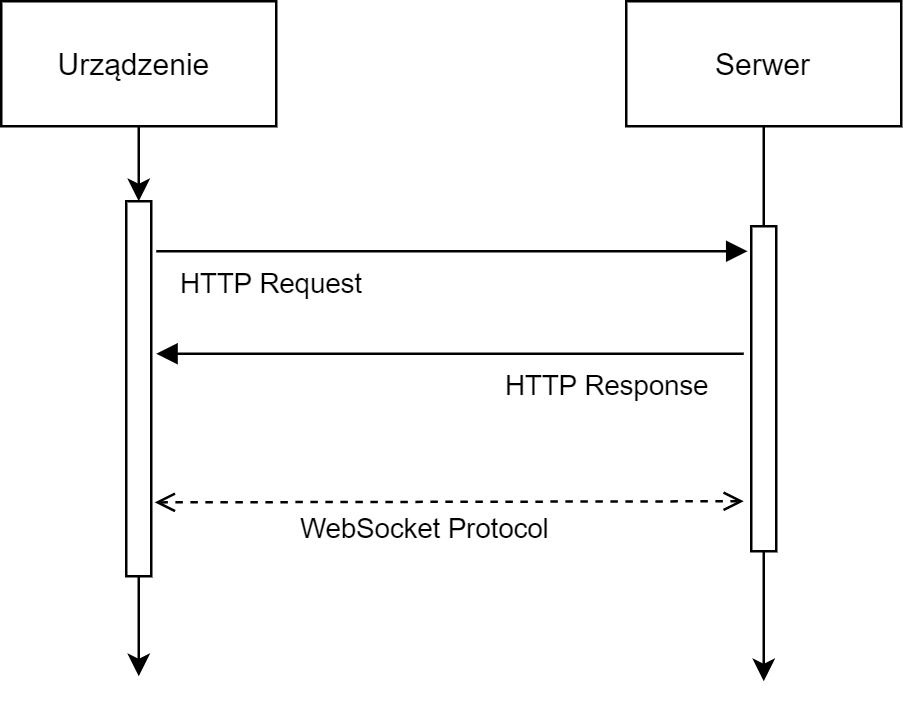
\includegraphics[width=\textwidth]{kp05}
    \caption{Placeholder}
    \label{fig:iotarch}
\end{figure}
\begin{itemize}
    \item Constrained Application Protocol (CoAP) to protokół warstwy aplikacji, który jest stosowany do urządzeń z ograniczonymi zasobami. Umożliwia komunikowanie się za pomocą podobnych protokołów oraz obsługuje multiemisjie.  CoAP został zaprojektowany do komunikację między urządzeniami w tej znajdującymi się w tej samej ograniczonej sieci.
\end{itemize}
